\chapter{Introducere}
\label{chap:introducere}

În cadrul acestei teme, am dorit simularea unui sistem de iluminare publică, cu ajutorul unui microcontroller de tip Arduino Mega. 
Cel mai comun tip de sistem pentru iluminat stradal întâlnit în România la momentul actual este alcătuit din lămpi, care în timpul zilei nu sunt puse în funcțiune, dar rămân aprinse pe toată durata nopții. Deși iluminatul stradal este necesar pe timpul nopții, metoda aceasta de implementare este foarte ineficientă. 
Sistemul propus va păstra utilitatea celui deja existent, dar va ajuta la optimizarea consumului de energie. În studiile din \cite{8539321,7513906}, bazate pe modele asemănătoare cu cel realizat de mine, implementarea unui astfel de sistem poate duce la scăderea consumului de energie electrică cu 40-45\%. Nu poate fi făcută o comparație directă din cauza diferențelor în logica de funcționare, dar câștigul tot poate fi estimat a fi semnificativ.  



\section{Formularea problemei generale}

Scopul lucrării este de a realiza un sistem alcătuit dintr-o serie de lămpi pentru iluminat stradal, care se aprind la intensitate mică doar când nivelul de luminozitate măsurat este destul de scăzut încât să poată fi considerat că este noapte. Tot pe timp de noapte, intrarea unui obiect în raza unui felinar duce la creșterea intensității luminii acestuia, în funcție de viteza obiectului. 

Obiectivele principale ale lucrării sunt implementarea practică a sistemului, analiza calitativă a funcționării acestuia și tratarea, măcar teoretică, a cazurilor excepționale pe care nu le-am realizat în practică din motive ce țin de limitări hardware, software sau de timp.

Este important de menționat faptul că, \textbf{pe durata nopții}, felinarele nu se vor stinge niciodată în întregime pentru sistemul realizat de mine. Deoarece acesta este cazul studiat cel mai mult, \textbf{orice mențiune a stingerii lor va însemna trecerea pe modul de intensitate minimă de funcționare}. Voi face diferențierea între cele două, în cazurile în care aceasta este relevantă.


Prezența vehiculelor este detectată cu ajutorul unor senzori de prezen\c{t}\u{a}
aflați între fiecare set de câte 2 felinare, iar acestea acționează astfel:

\begin{itemize}
    \item  La momentul depășirii de către vehicul al unui senzor, felinarul următor se va aprinde, gradul de luminozitate urm\^{a}nd sa fie ales în funcție de viteza automobilului;
    \item  Felinarul anterior acestuia urmează să se stingă, gradual.
\end{itemize}

În următoarele imagini este prezentat modul dorit de funcționare pentru cazul simplu al trecerii unui singur vehicul, în soluția propusă de mine pentru realizarea sistemului. La depășirea primilor 2 senzori se va aprinde primul felinar, în concordanță cu viteza calculată, după cum arată \figref{fig:car1}.
  
 \begin{figure}[!ht]
    \begin{center}
    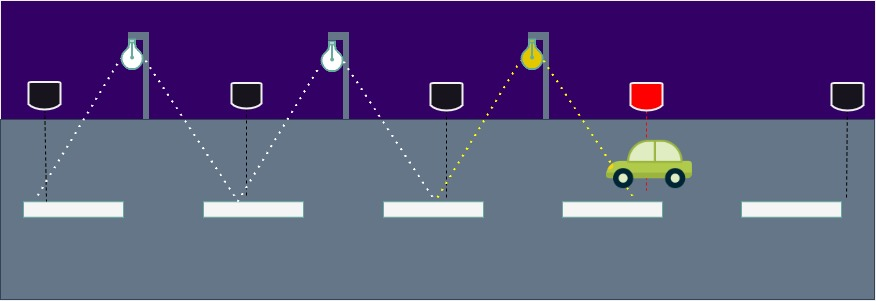
\includegraphics[width=0.9\linewidth,keepaspectratio]{pics/cardraw1.jpg}
    \end{center}
    \caption{Intrare vehicul în sistem}
    \label{fig:car1}
\end{figure}

Trecerea de următorul senzor, prezentată în \figref{fig:car2}, duce la aprinderea următorului felinar, în timp ce nivelul de luminozitate al celui anterior începe să scadă treptat.

 \begin{figure}[!ht]
    \begin{center}
    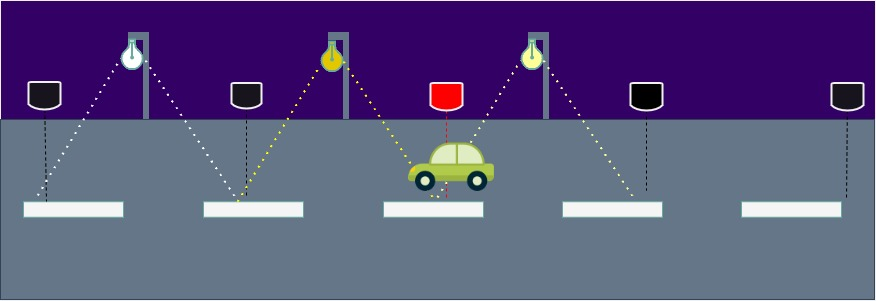
\includegraphics[width=0.9\linewidth,keepaspectratio]{pics/cardraw2.jpg}
    \end{center}
    \caption{Vehicul în stare intermediară}
    \label{fig:car2}
\end{figure}

În \figref{fig:car3} am surprins momentul ieșirii vehiculului din sistem, în care ultimul felinar începe să se stingă, cel anterior încă nu a avut timp să se stingă complet, iar primul deja a revenit la starea inițială.

 \begin{figure}[!ht]
    \begin{center}
    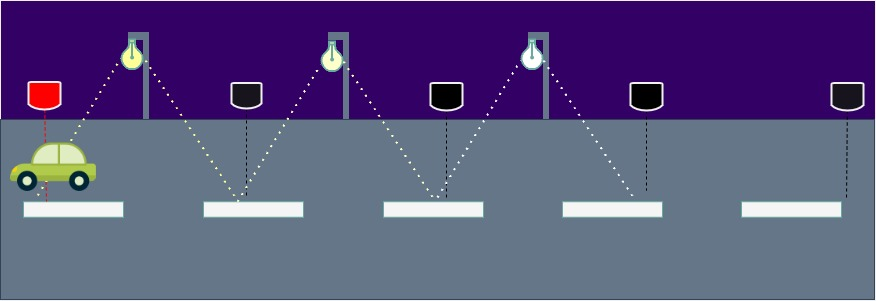
\includegraphics[width=0.9\linewidth,keepaspectratio]{pics/cardraw3.jpg}
    \end{center}
    \caption{Vehicul ieșind din porțiunea reprezentată}
    \label{fig:car3}
\end{figure}
